%%
% Interação e Deteção de Partículas - MIEF
% Problema 3 - 
%
% Data: 03/11/2021


\documentclass[a4paper, 12pt]{article} % Set to article class
\usepackage[portuguese]{babel} % Set language to portuguese

\usepackage{lmodern} % Changes to a cleaner font
\usepackage{listings}
\usepackage{color}


\usepackage[T1]{fontenc} % Add support to language
\usepackage[cp1252, utf8]{inputenc} % Add support to language

\chardef\_=`_ % Add support to underscores
\usepackage{graphicx, epstopdf, rotating, % Graphics support
	array, booktabs, float, % Tables packages
	makecell, enumitem, 
	amsmath, amssymb, % Better math print
	siunitx % Plot support	
} % Add basic support

\usepackage[bookmarks, pdftex, hidelinks]{hyperref} % Add hidden bookmarks
\usepackage[margin = .75in]{geometry} % Tool to remove margins
\graphicspath{{images/}} % Add path to images folder

\renewcommand\theadfont{\bfseries} % Make table headers better
\setlength\parindent{0pt} % Remove paragraph indent
\pagestyle{plain} % Adds custom page style
\usepackage[font=small]{caption} % Change caption size

% Nome da disciplina
\def\classtitle{Interação e Deteção de Partículas}

% Nome do relatório
\def\worktitle{Projeto Final - Terapia de Protões}

% Nome do/a professor/a
\def\profname{Doutor Alexandre Lindote}

% Nome do local 
\def\worklocal{Universidade de Coimbra}

% Data do trabalho
\def\workdate{\today}

% Nome dos autores
\def\authors{
	José Nuno da Cruz Faria - 2015252736
}

% Turma
\def\classinfo{Teórica Prática, Turma PL1}

\renewcommand\thesection{\arabic{section})}

% Resize matrice lines
\makeatletter
\renewcommand*\env@matrix[1][\arraystretch]{%
  \edef\arraystretch{#1}%
  \hskip -\arraycolsep
  \let\@ifnextchar\new@ifnextchar
  \array{*\c@MaxMatrixCols c}}
\makeatother

\definecolor{clr-background}{RGB}{255,255,255}
\definecolor{clr-text}{RGB}{0,0,0}
\definecolor{clr-string}{RGB}{163,21,21}
\definecolor{clr-namespace}{RGB}{0,0,0}
\definecolor{clr-preprocessor}{RGB}{128,128,128}
\definecolor{clr-keyword}{RGB}{0,0,255}
\definecolor{clr-type}{RGB}{43,145,175}
\definecolor{clr-variable}{RGB}{0,0,0}
\definecolor{clr-constant}{RGB}{111,0,138} % macro color
\definecolor{clr-comment}{RGB}{0,128,0}

\lstdefinestyle{VS2017}{
	backgroundcolor=\color{clr-background}\ttfamily,
	basicstyle=\color{clr-text}\ttfamily, % any text
	stringstyle=\color{clr-string}\ttfamily,
	identifierstyle=\color{clr-variable}\ttfamily, % just about anything that isn't a directive, comment, string or known type
	commentstyle=\color{clr-comment}\ttfamily,
	directivestyle=\color{clr-preprocessor}\ttfamily, % preprocessor commands
	% listings doesn't differentiate between types and keywords (e.g. int vs return)
	% use the user types color
	keywordstyle=\color{clr-type}\ttfamily,
	%keywordstyle={\color{clr-constant}}\ttfamily, % you'll need to define these or use a custom language
	tabsize=4
}


\lstset{language=C++,
                style=VS2017
}


\begin{document}
	
	\begin{figure}[t] % Add logo
		\centering
		
\includegraphics[width=0.85\linewidth]{uc_fctuc}
	\end{figure}

	\vspace*{0.05\textheight}	
	\begin{table}[!htbp]
		\centering
		
		{\Huge \classtitle}\\
		
		\vspace*{0.01\textheight}
		{\Large \textbf{\worktitle}}\\
		
		\vspace*{0.02\textheight}
		{\large {\worklocal, \workdate}}
		
	\end{table}
	
	\begin{table}[H]
		\begin{center}
			{\normalsize % Mudar a fonte para mais pequena(?)
				\textbf\classinfo\\
				\emph{Prof. \profname}\\ 
				\vspace{0.0035\textheight}			
				\authors 
			}
		\end{center}
	\end{table}

	\section{Introdução}

	A passagem de partículas carregadas pela matéria pode ser descrita através de dois fenómenos: perda de energia da partícula, e desvio da trajetória da partícula.
	Existem diversos processos físicos que causam estes efeitos (Bremsstrahlung, reações nucleares, emissão de radiação de Cherenkov), mas é principalmente causado por \cite{Leo}:

	\begin{itemize}
		\item colisões inelasticas com os eletróes atómicos do material do alvo;
		\item \textit{scattering} elástico com o núcleo.
	\end{itemize}
    
	A perda energética de uma partícula a atravessar um dado material é descrito pelo seu potencial de travagem ($dE/dx$). Figura \ref{fig:bethe} mostra a variação do potencial de travagem para diferentes particulas. 

	\begin{figure}[H]
		\centering
		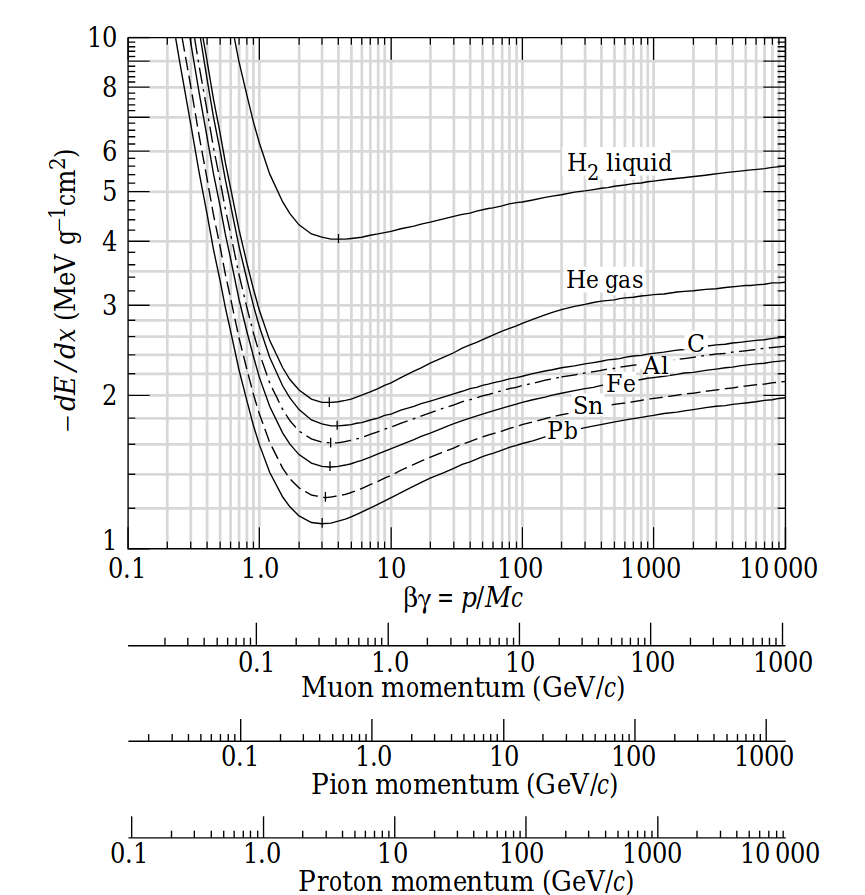
\includegraphics[width=0.5\linewidth]{bethe_bloch.png}
		\caption{Variação de -dE/dx em função de $\beta\gamma$ para diferentes partículas.}
		\label{fig:bethe}
	\end{figure}

	Para partículas pesadas carregadas (\textit{e.g.} protões, iões), o potencial de travagem pode ser descrito pela equação de Bethe-Block (sem correções de densidade e de camada), para $0.1 < \beta\gamma < 1000 $:

	\begin{equation}
		-\frac{dE}{dx} = K \rho \frac{Z_{alvo}}{A_{alvo}} \frac{z^2}{\beta^2}\Bigg[ \ln \Big(\frac{2 m_e \gamma^2 \nu^2 W_{max}}{I^2}\Big) - 2\beta^2 \Bigg]
		\label{eq:bethe_block}
	\end{equation}

	onde $K = 2\pi N_a r_e^2 m_e c^2 = 0.1535\ \text{MeV cm}^2/\text{g}$, $\rho$ é a densidade do material do alvo, $Z_{alvo}$ e $A_{alvo}$ são o número atómico e massa atómica respetivamente, $z$ é a carga da partícula incidente (em unidades de $e$), $\beta$ é a velocidade relativa da partícula ($\beta=v/c$), $\gamma$ é o fator de Lorentz, $I$ é o potencial de excitação médio, e $W_{max}$ é a energia máxima que pode ser transferida numa única colisão.

	\paragraph{} Podemos observar que o potencial de travagem que para energias não relativistas, a expressão é principalmente dominada pelo termo $1/\beta^2$, logo aumenta com a diminuição da velocidade. Isto significa que à medida que a partícula atravessa a materia, ela abranda devido às interações eletromagnéticas, que por sua vez aumenta o potencial de travagem, portanto deveremos observar a maioria da sua energia depositada no final da trajetoria da partícula. Este efeito é chamado de pico de Bragg, e é extremamente utilizado em aplicações médicas onde pretendemos depositar uma alta dose de radiação em tumores com o mínimo de destruição do tecido envolvente.

	\paragraph{} Neste trabalho iremos efetuar uma simulação da interação de feixe de protões com tecido mole, com o objetivo de determinar a energia necessária para o feixe depositar a energia num tumor que encontra-se 7 cm em profundidade da superfície do tecido. Foram efetuadas no total 11 simulações, uma por cada energia média diferente do feixe (de 50 a 150 MeV, em passos de 10 MeV).

	\section{Simulador}
	O código para o simulador de Monte-Carlo foi criado em Geant4 com base no \textit{template} fornecido\footnote{\url{https://lip.pt/~alex/G4Classes/Examples/BraggPeak.zip}}, e encontra-se no seguinte URL: \url{https://github.com/jncfa/idp_exercices/tree/master/final_project}.

	\paragraph{} Para criar o simulador é necessário adicionar 3 componentes ao \textit{template}:
	
	\begin{enumerate}
		\item Geometria da Simulação: Definir a posição e orientação de cada componente a simular, \textit{i.e.} posição e orientação do alvo de ``tecido mole''.
		\item Gerador da Partículas Primárias: Definir quais são as partículas emitidas e as suas propriedades (\textit{i.e.} energia, posição, e orientação de cada partícula).
		\item Recolha de informação para análise: Definir um mecanismo que permita a recolha dos dados da simulação.
	\end{enumerate}

	\paragraph{} Fora estas componentes, foi também necessário alterar a \texttt{PhysicsList} que define as interações físicas que serão simuladas, tendo sido usado a \texttt{PhysicsList} que vinha previamente configurada no \textit{template}, para ter um corte de 0.01 mm.

	\paragraph{} Nas próximas secções, é detalhada a implementação de cada componente.
	
	\subsection{Geometria da Simulação}
	Para definir a geometria da simulação, utilizámos a classe \texttt{G4VUserDetectorConstruction}\footnote{\url{https://apc.u-paris.fr/~franco/g4doxy4.10/html/class_g4_v_user_detector_construction.html}} para definir a posição, orientação dos materiais que compõe o nosso alvo. Foi usado um dos tecidos moles que encontrava-se na lista NIST de materiais, com o código \texttt{G4\_TISSUE\_SOFT\_ICRP}, com densidade $\rho=1.03\ g/cm^3$.

	\begin{lstlisting}[language=C++]
// Inicia o G4NistManager e procura pelo material G4_TISSUE_SOFT_ICRP
G4NistManager* manager = G4NistManager::Instance();
G4Material* softTissue = manager->FindOrBuildMaterial(
	"G4_TISSUE_SOFT_ICRP");
	\end{lstlisting}

	A dimensão do alvo tem a largura e altura do ``mundo'' da simulação e uma profundidade de 5 m (que é muito maior do que o alcance médio dos protões para o espetro de energias que iremos simular). O material que compõe o ambiente envolvente é vácuo, de modo a considerarmos apenas as interações com o alvo.  

	\begin{lstlisting}[language=C++]
// Tamanho do mundo da simulacao
G4double fWorldLength= 10.0*m;
G4double HalfWorldLength = 0.5*fWorldLength;
// Espessura do alvo
G4double targetThickness = 5*m;
// Criar alvo com o dado tamanho e material
G4Box* solidTarget = new G4Box("target",0.5*targetThickness,
	HalfWorldLength,HalfWorldLength);
G4LogicalVolume* logicTarget = new G4LogicalVolume(solidTarget,
	softTissue,"Target",0,0,0);
G4ThreeVector pos = G4ThreeVector(0.5*targetThickness,0,0);
G4VPhysicalVolume* physiTarget = new G4PVPlacement(0, pos, 
	logicTarget, "Target", logicWorld, false, 0);	
	\end{lstlisting}

\subsection{Gerador da Partículas Primárias}
	Para definir as partículas que são geradas na simulação, utiliza-se uma classe do tipo \\\texttt{G4VUserPrimaryGeneratorAction}\footnote{\url{https://apc.u-paris.fr/~franco/g4doxy4.10/html/class_g4_v_user_primary_generator_action.html}} para definir o evento de ``geração'' de partículas. Nessa classe, é criada uma \texttt{G4ParticuleGun}\footnote{\url{https://apc.u-paris.fr/~franco/g4doxy/html/classG4ParticleGun.html}} que emite um protão.

	\begin{lstlisting}[language=C++]
// Criar uma particle gun de uma particula
G4ParticleGun particleGun = new G4ParticleGun(1);
// Obter informacao dos protoes
G4ParticleTable *particleTable = 
	G4ParticleTable::GetParticleTable();
G4ParticleDefinition *particle = 
	particleTable->FindParticle("proton");
particleGun->SetParticleDefinition(particle);
// Definir posicao, orientacao e momento da particula 
// (igual para todas as particulas)
particleGun->SetParticleMomentumDirection(
	G4ThreeVector(1., 0., 0.));
particleGun->SetParticlePosition(
	G4ThreeVector(-1*m, 0. * cm, 0. * cm));
	\end{lstlisting}

	Para a nossa simulação, considerámos que o feixe de protões tem uma distribuição energética que segue uma distribuição Gaussiana, com $\sigma=2\%$ e $\mu=\{50,60,\dots, 150\}\ \text{MeV}$, onde efetuamos uma simulação para cada valor diferente da energia média do feixe. O valor foi gerado aleatóriamente utilizado o método de Box-Muller, para cada partícula do feixe.

	\begin{lstlisting}[language=C++]
// Distribuicao Normal (mu=1, std=0) usando metodo de Box-Muller
G4float Z = pow((-2*log(G4UniformRand())), 0.5) * 
	cos(2*M_PI*G4UniformRand());
// Media e desvio padrao que sao pretendidos 
G4float mean_value = 100*MeV;
G4float std = 0.02;
particleGun->SetParticleEnergy(Z*std*mean_value + mean_value);
	\end{lstlisting}

	\subsection{Recolha informação para análise}
	Para recolher os dados da simulação, criamos uma classe do tipo \texttt{G4UserSteppingAction}\footnote{\url{https://apc.u-paris.fr/~franco/g4doxy/html/classG4UserSteppingAction.html}} que é chamada a cada passo da iteração da simulação.

	\paragraph{} Em cada passo, o programa verifica se a partícula que está a ser seguida neste passo encontra-se no volume do detector, e se é uma partícula primária e obtem a energia que foi depositada nessa interação, a profundidade a que a partícula se encontra e a variação de posição simulada nesta iteração, registando os valores no ficheiro ``BraggPeak.out''.
	

	\begin{lstlisting}[language=C++]
// {Na inicializacao da classe...}
std::ofstream bout;
bout.open("BraggPeak.out");
// {Codigo chamado a cada passo...}
G4Track* thisTrack = thisStep->GetTrack();
G4VPhysicalVolume* theVolume = thisTrack->GetVolume();
// Ver se evento aconteceu no alvo e se foi com uma particula 
// primaria (i.e. nao tem parent track)
const G4ParticleDefinition* thisParticle = 
	thisTrack->GetParticleDefinition();
if(theVolume->GetName() == "Target" && 
	thisParticle->GetParticleName() == "proton"){
	bout << thisTrack->GetTrackLength() / cm << "\t"
			<< thisStep->GetTotalEnergyDeposit() /MeV << "\t"
			<< thisStep->GetStepLength() / cm << G4endl;
}

	\end{lstlisting}
	

	\section{Resultados obtidos e Discussão}
	Como mencionado previamente, efetuamos uma simulação ($n=10000$ partículas emitidas em cada simulação) para cada valor de energia média do feixe (50 até 150 MeV, em passos de 10 MeV). As figuras seguintes mostram a dosagem medida em função da profundidade para cada energia média inicial do feixe.

	\begin{figure}[H]
		\begin{minipage}[r]{.49\linewidth}
			\centering
			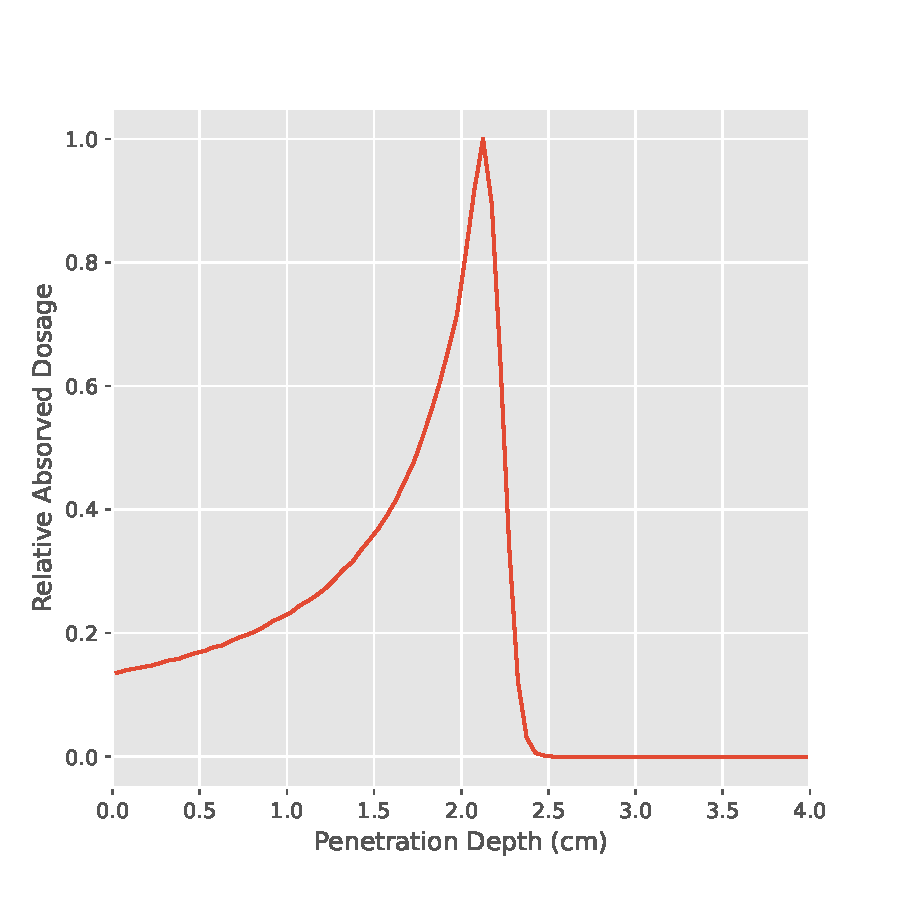
\includegraphics[width=\linewidth]{bragg_peak_50mev.pdf}
			\caption{Dosagem medida em função da profundidade para um feixe com energia média de 50 MeV. O pico da dosagem é observado a uma profundidade de $2.13 \pm 0.05$ cm.}
			\label{fig:bragg_peak50}
		\end{minipage}
		\hspace{.01\linewidth}
		\begin{minipage}[r]{.49\linewidth}
			\centering
			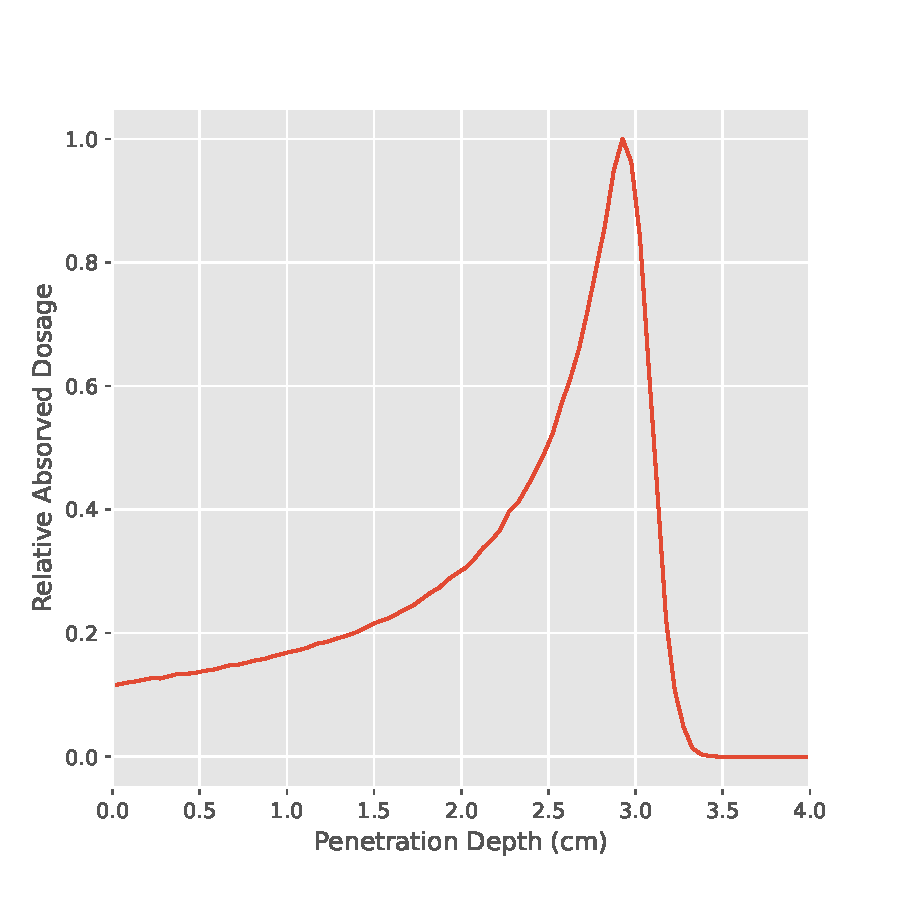
\includegraphics[width=\linewidth]{bragg_peak_60mev.pdf}
			\caption{Dosagem medida em função da profundidade para um feixe com energia média de 60 MeV. O pico da dosagem é observado a uma profundidade de $2.93 \pm 0.05$ cm.}
			\label{fig:bragg_peak60}
		\end{minipage}
	\end{figure}
	\begin{figure}[H]
		\begin{minipage}[r]{.49\linewidth}
			\centering
			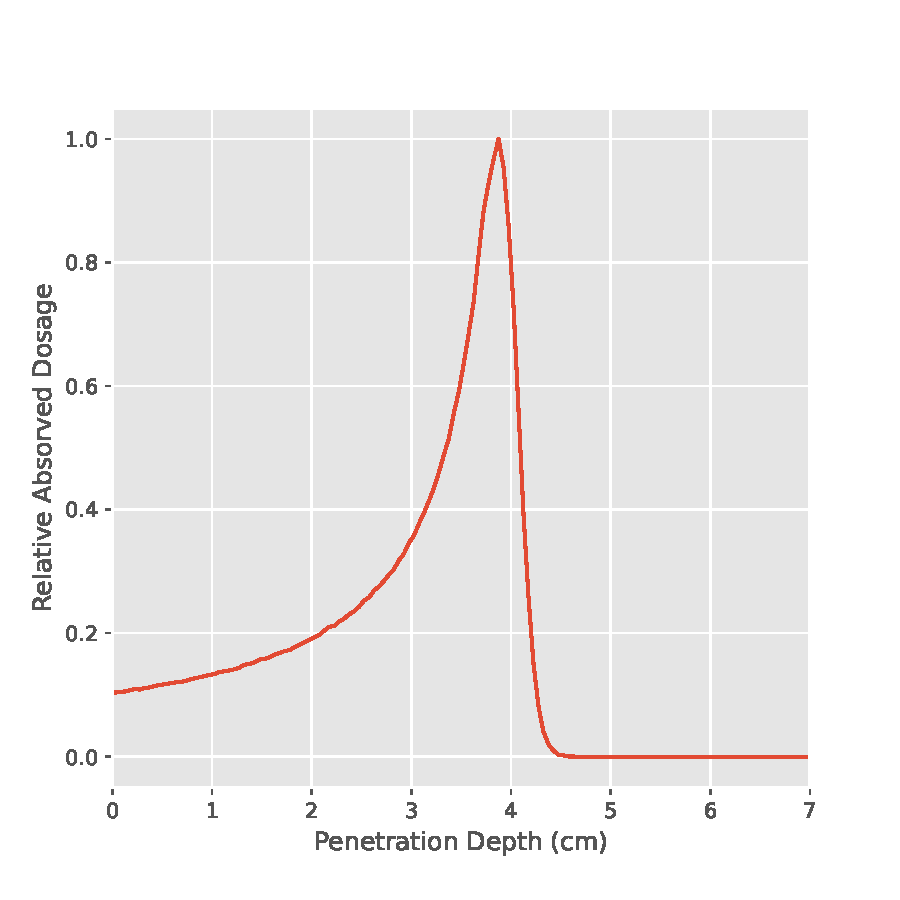
\includegraphics[width=\linewidth]{bragg_peak_70mev.pdf}
			\caption{Dosagem medida em função da profundidade para um feixe com energia média de 70 MeV. O pico da dosagem é observado a uma profundidade de $3.88 \pm 0.05$ cm.}
			\label{fig:bragg_peak70}
		\end{minipage}
		\hspace{.01\linewidth}
		\begin{minipage}[r]{.49\linewidth}
			\centering
			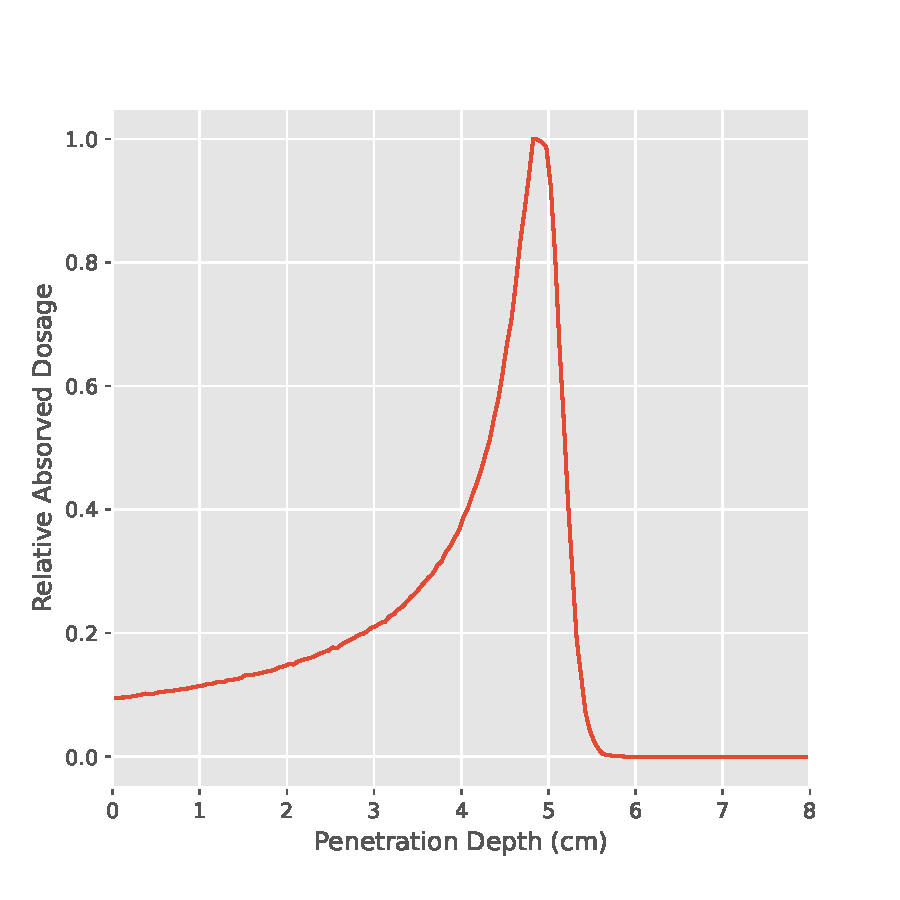
\includegraphics[width=\linewidth]{bragg_peak_80mev.pdf}
			\caption{Dosagem medida em função da profundidade para um feixe com energia média de 80 MeV. O pico da dosagem é observado a uma profundidade de $4.83 \pm 0.05$ cm.}
			\label{fig:bragg_peak80}
		\end{minipage}
	\end{figure}
	\begin{figure}[H]
		\begin{minipage}[r]{.49\linewidth}
			\centering
			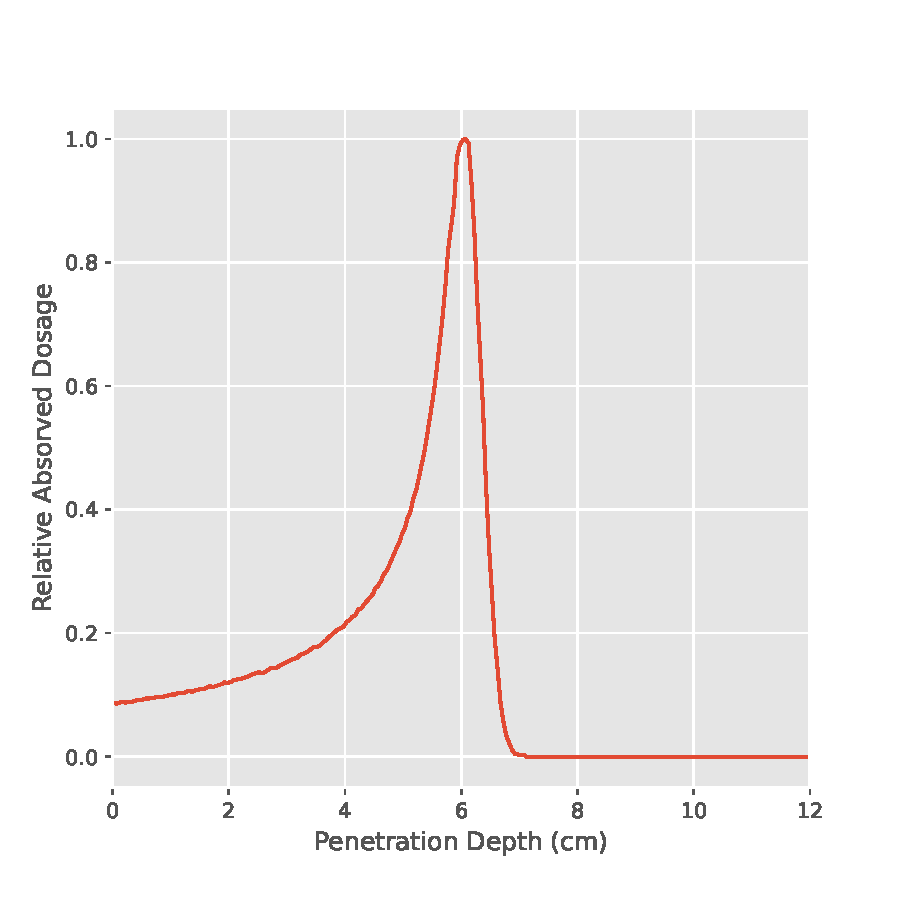
\includegraphics[width=\linewidth]{bragg_peak_90mev.pdf}
			\caption{Dosagem medida em função da profundidade para um feixe com energia média de 90 MeV. O pico da dosagem é observado a uma profundidade de $6.08 \pm 0.05$ cm.}
			\label{fig:bragg_peak90}
		\end{minipage}
		\hspace{.01\linewidth}
		\begin{minipage}[r]{.49\linewidth}
			\centering
			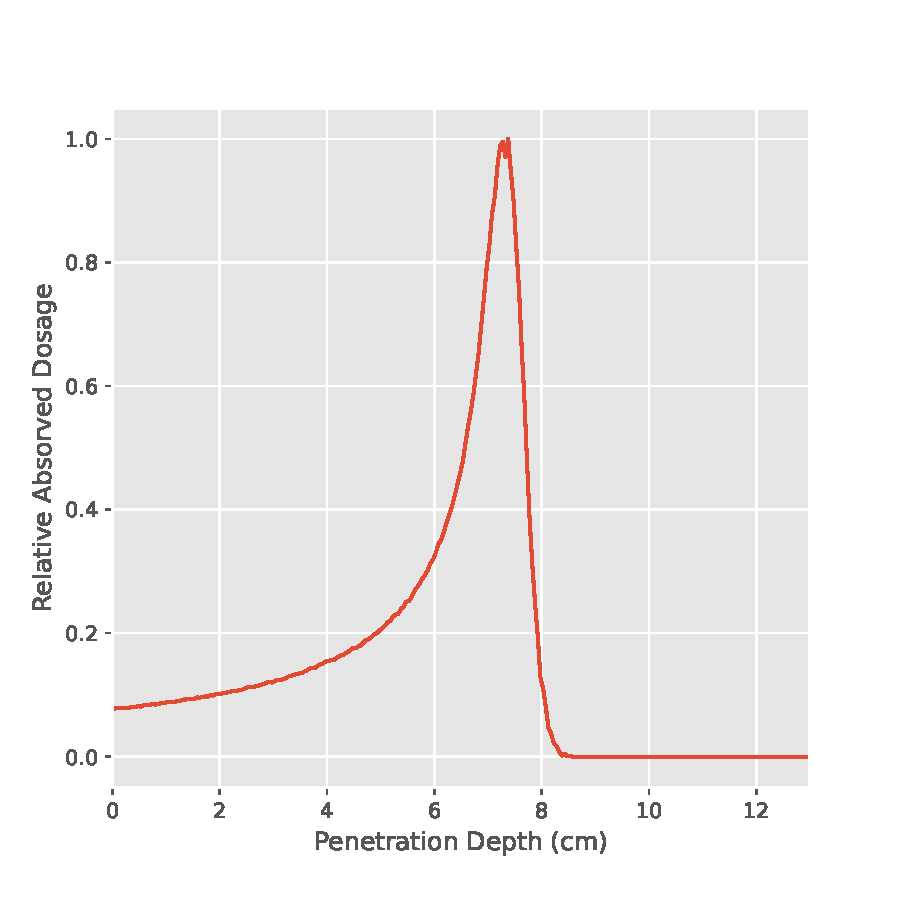
\includegraphics[width=\linewidth]{bragg_peak_100mev.pdf}
			\caption{Dosagem medida em função da profundidade para um feixe com energia média de 100 MeV. O pico da dosagem é observado a uma profundidade de $7.38  \pm 0.05$ cm.}
			\label{fig:bragg_peak100}
		\end{minipage}
	\end{figure}
	\begin{figure}[H]
		\begin{minipage}[r]{.49\linewidth}
			\centering
			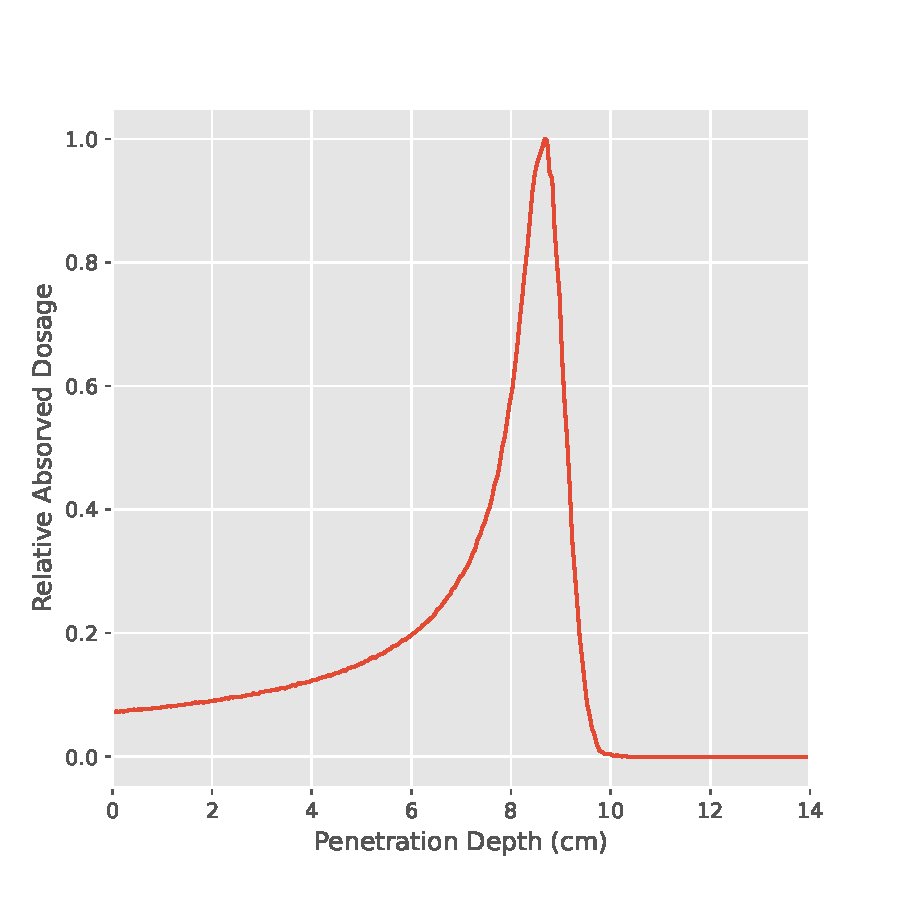
\includegraphics[width=\linewidth]{bragg_peak_110mev.pdf}
			\caption{Dosagem medida em função da profundidade para um feixe com energia média de 110 MeV. O pico da dosagem é observado a uma profundidade de $8.68  \pm 0.05$ cm.}
			\label{fig:bragg_peak110}
		\end{minipage}
		\hspace{.01\linewidth}
		\begin{minipage}[r]{.49\linewidth}
			\centering
			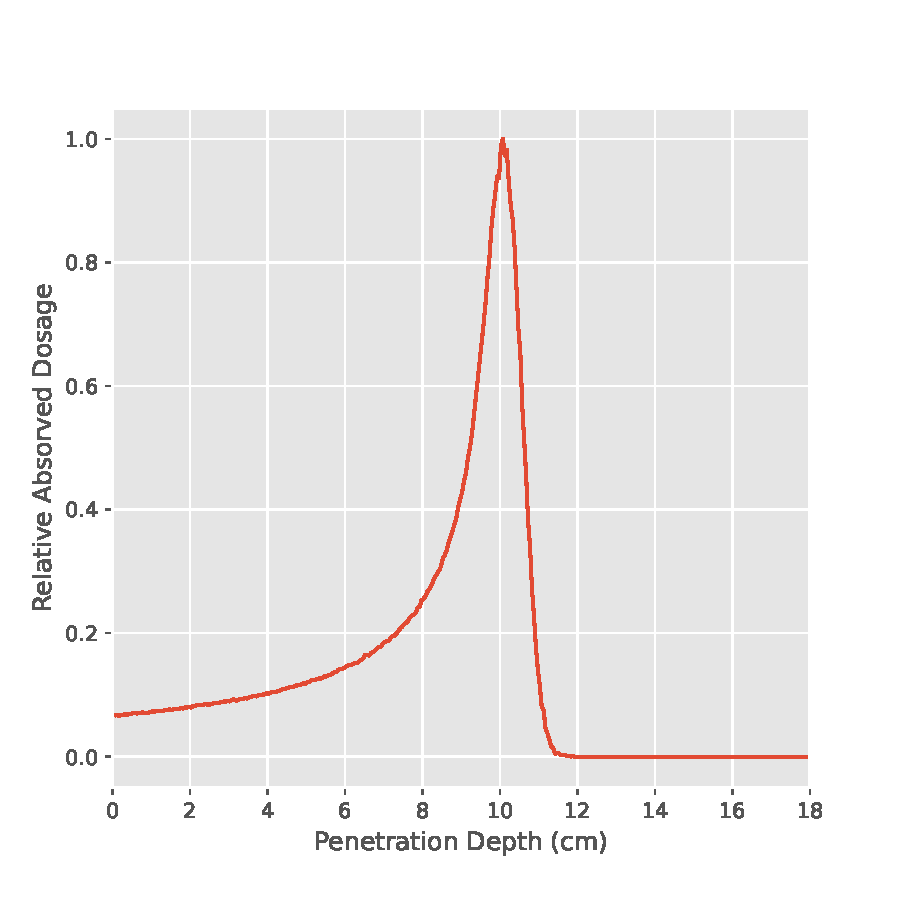
\includegraphics[width=\linewidth]{bragg_peak_120mev.pdf}
			\caption{Dosagem medida em função da profundidade para um feixe com energia média de 120 MeV. O pico da dosagem é observado a uma profundidade de $10.08 \pm 0.05$ cm.}
			\label{fig:bragg_peak120}
		\end{minipage}
	\end{figure}
	\begin{figure}[H]
		\begin{minipage}[r]{.49\linewidth}
			\centering
			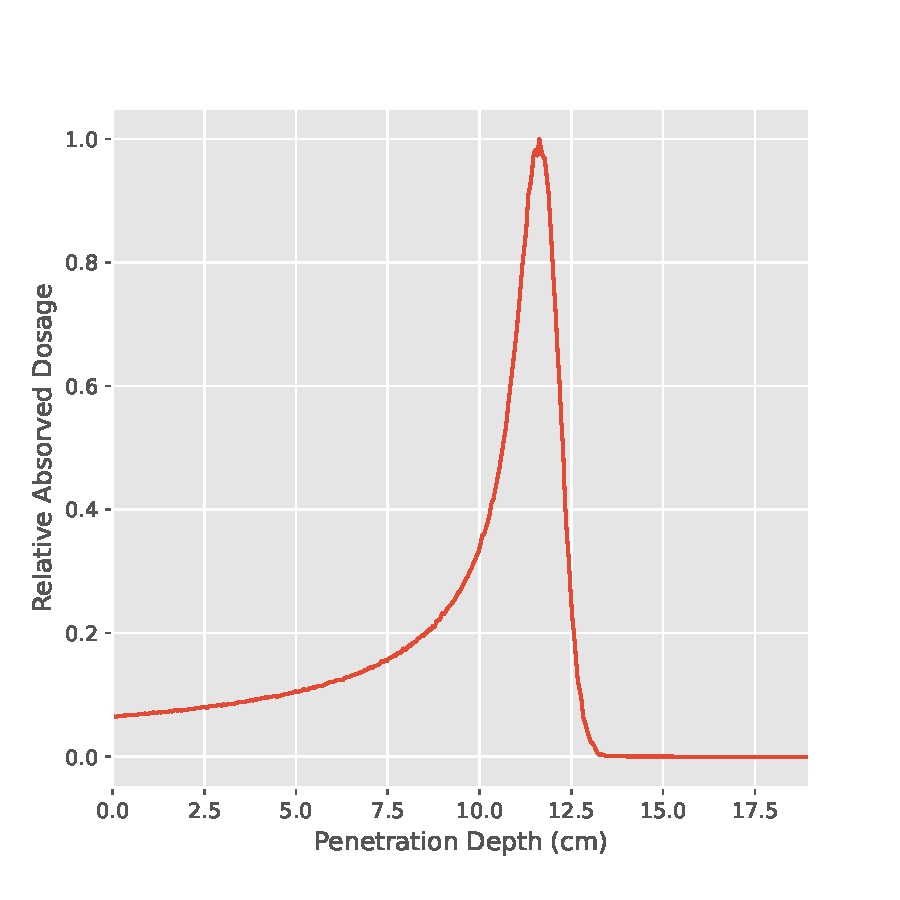
\includegraphics[width=\linewidth]{bragg_peak_130mev.pdf}
			\caption{Dosagem medida em função da profundidade para um feixe com energia média de 130 MeV. O pico da dosagem é observado a uma profundidade de $11.63  \pm 0.05$ cm.}
			\label{fig:bragg_peak130}
		\end{minipage}
		\hspace{.01\linewidth}
		\begin{minipage}[r]{.49\linewidth}
			\centering
			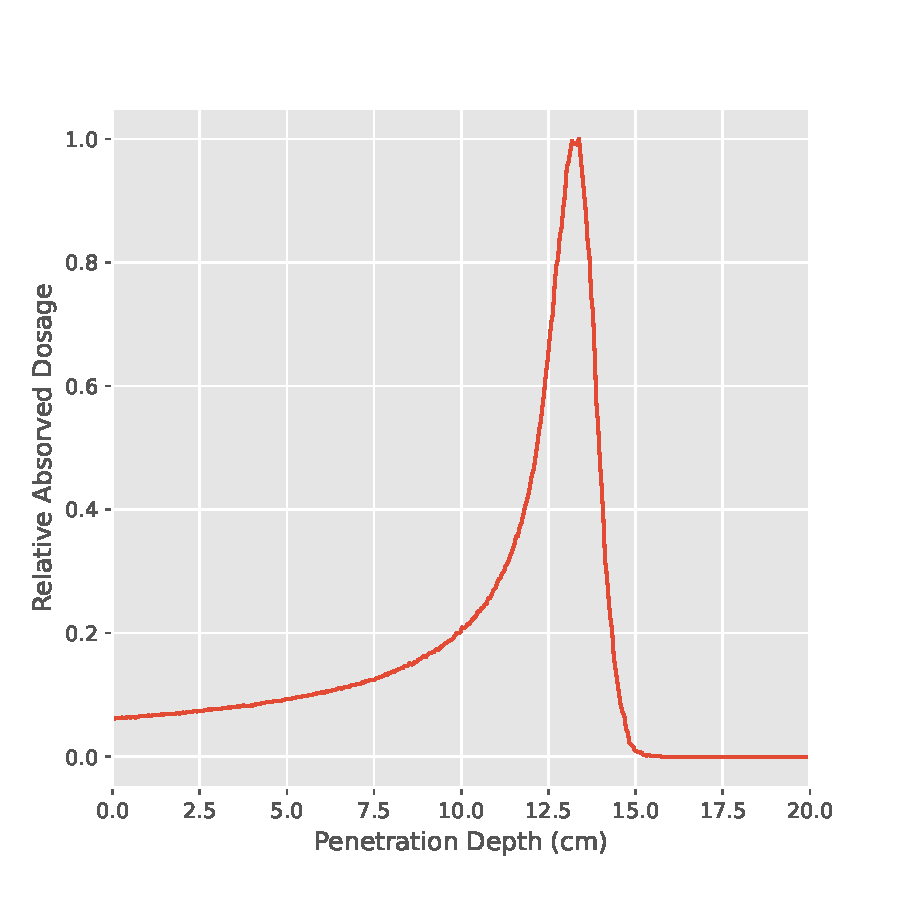
\includegraphics[width=\linewidth]{bragg_peak_140mev.pdf}
			\caption{Dosagem medida em função da profundidade para um feixe com energia média de 140 MeV. O pico da dosagem é observado a uma profundidade de $13.38  \pm 0.05$ cm.}
			\label{fig:bragg_peak140}
		\end{minipage}
	\end{figure}
	\begin{figure}[H]
		\centering
		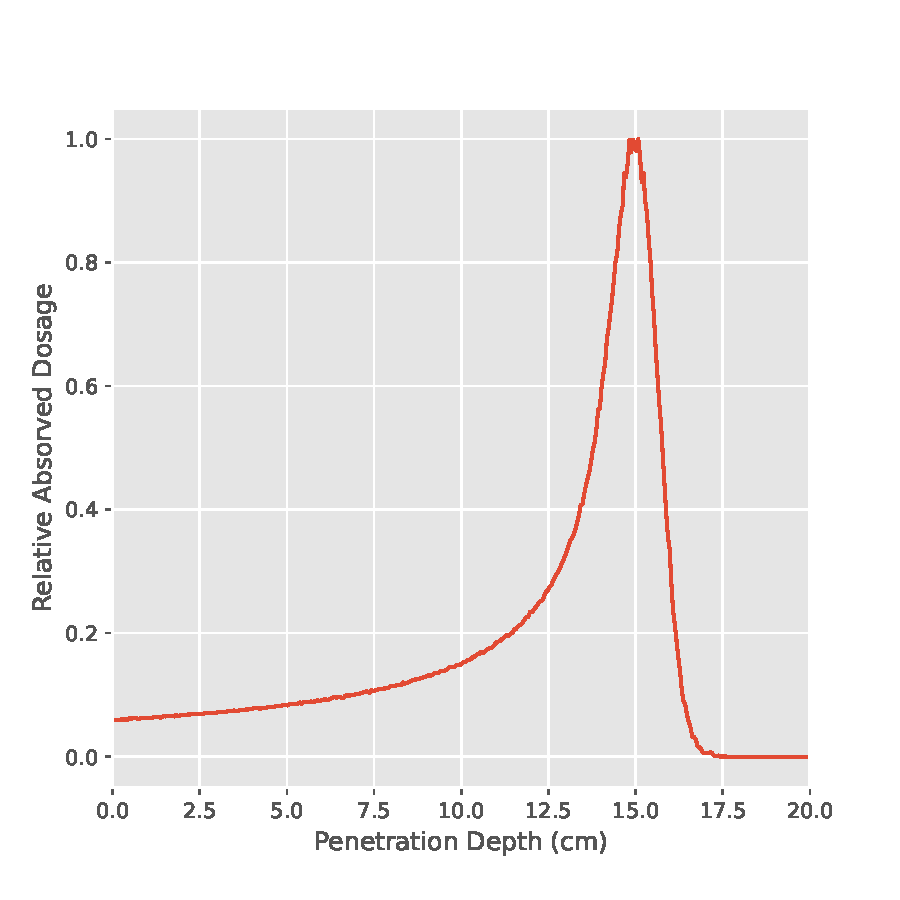
\includegraphics[width=0.5\linewidth]{bragg_peak_150mev.pdf}
		\caption{Dosagem medida em função da profundidade para um feixe com energia média de 150 MeV. O pico da dosagem é observado a uma profundidade de $15.08 \pm 0.05$ cm.}
		\label{fig:bragg_peak150}
	\end{figure}

	\paragraph{} Para estimar a energia do feixe para tratar um tumor a 7 cm de profundidade, utilizámos os picos obtidos anteriormente para efetuar uma interpolação linear para obter o valor de energia médio associado, obtendo uma energia de $E=97.12 \pm 0.30$ MeV para tratar o tumor minimizando a destruição do tecido envolvente.

	\begin{figure}[H]
		\centering
		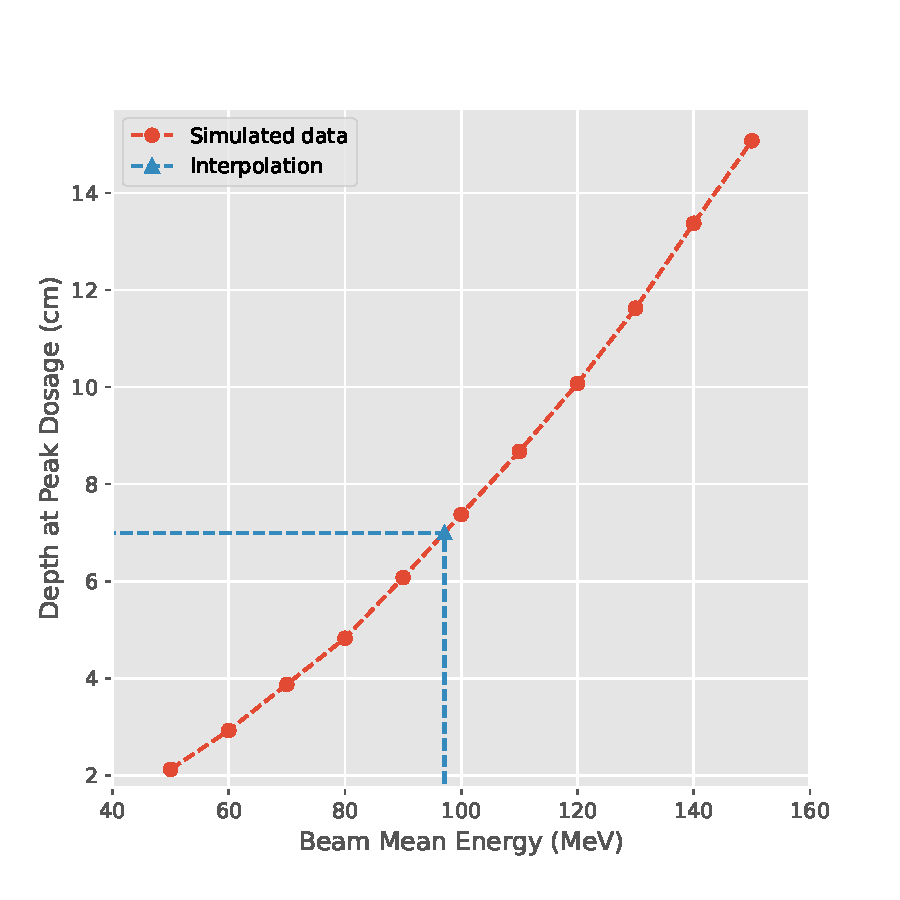
\includegraphics[width=.5\linewidth]{bragg_peak_interp.pdf}
		\caption[Pontos médios dos picos de Bragg obtidos em função da energia média inicial do feixe de protões.]{Pontos médios dos picos de Bragg obtidos em função da energia média do feixe de protões. O ponto correspondente a 7cm está também marcado no gráfico, sendo obtido através de uma interpolação linear com os pontos de 90 e 100 MeV, correspondendo a uma energia de $97.12 \pm 0.30$ MeV\footnotemark. }
		\label{fig:bragg_peak_adjusted}
	\end{figure}
	\footnotetext{O erro foi obtido através da fórmula de propagação de erro: $\sigma f(x_1,x_2,\dots)^2 = \sum_n\Big(\sigma x_n \frac{\partial f}{\partial x_n}\Big)^2$.}
	Dependendo da dimensão do tumor, poderá ser necessário modelar a distribuição energética do feixe para ter um \textit{spread-out Bragg peak} (SOBP), de modo atingir o tumor inteiro.

	\bibliographystyle{IEEEtran}
	\bibliography{references}
\end{document}